% =============================================================================
\chapter{Squeezing in 3D BEC interferometry}
\label{cha:bec-squeezing}
% =============================================================================

This chapter contains squeezing results from \cite{Opanchuk2012}.


\copypaste{copypaste begins}

The Wigner method is able to predict not only the average values of different observables,
but their variances too.
As an example, we now calculate the degree of squeezing $\xi^2$, introduced in~\cite{Wineland1994,Sorensen2001}.
This allows the analysis of experiments beyond the usual shot noise limit~\cite{Riedel2010,Gross2010}.
If we define spin component operators as
$\hat{S}_{x} = [ \hat{S}_+ + \hat{S}_+^\dagger ] / 2 $,
$\hat{S}_{y} = i [ \hat{S}_+ - \hat{S}_+^\dagger ] / 2 $ and
\begin{equation}
\begin{split}
    \hat{S}_+ & = \int \upd^D\xvec \left[
        \widehat{\Psi}^\dagger_2 (\xvec) \widehat{\Psi}_1 (\xvec)
    \right], \\
    \hat{S}_z & = \frac{1}{2} \int \upd^D\xvec \left[
        \widehat{\Psi}^\dagger_1 (\xvec) \widehat{\Psi}_1 (\xvec)
        - \widehat{\Psi}^\dagger_2 (\xvec) \widehat{\Psi}_2 (\xvec)
    \right],
\end{split}
\end{equation}
the average values of spin vector components can be calculated similarly to the average density in
eq.~(\ref{eqn:wigner-density}).
Now we can shift the centre of coordinates to the end of the vector
$\langle \mathbf{S} \rangle = \{ \langle \hat{S}_x \rangle, \langle \hat{S}_y \rangle, \langle \hat{S}_z \rangle \}$
and rotate it, making the $z^\prime$-axis parallel to $\mathbf{S}$ and choosing the remaining axes $x^\prime$ and $y^\prime$ so that
$\Delta \hat{S}^2_{y^\prime} $ is minimized.

Second-order moments of spin operators are represented using fourth-order moments of field operators
and, therefore, can be calculated using wavefunctions in Wigner representation.
In this new coordinate system the squeezing parameter is expressed simply as
\begin{equation}
\label{eqn:squeezing}
    \xi^2 = \frac{N \Delta \hat{S}^2_{y^\prime}}{\langle S \rangle^2},
\end{equation}
where $N$ is the total number of atoms.
The formula for the squeezing parameter in the original coordinate system can be found elsewhere~\cite{Li2009}.
The squeezing parameter serves as a measure of atomic entanglement in the condensate,
when the atoms are entangled if $\xi^2 < 1$~\cite{Sorensen2001}.

\copypaste{copypaste ends}

% =============================================================================
\section{Moments of field operator in Wigner representation}
% =============================================================================


This chapter shows how to calculate different kinds of observables from wavefunctions in Wigner representation.
From the definition of Wigner function~\cite{Gardiner2004}:
\[
	\langle \symprod{ \hat{a}^r ( \hat{a}^\dagger)^s } \rangle
	= \int \alpha^r (\alpha^*)^s W (\alpha, \alpha^*) d^2\alpha ,
\]
where $\{\}_{\mathrm{sym}}$ stands for symmetrically ordered operator product.
It can be shown that similar relation applies for the multimode field operator:
\[
	\langle \symprod{ \Psiop^r ( \Psiop^\dagger)^s } \rangle
	= \int \Psi^r (\Psi^*)^s W (\Psi, \Psi^*) \delta^2\Psi.
\]
This equation can be further generalised for multi-component field.
In simulations, Wigner function $W$ can be treated as the probability distribution, allowing to replace the integral by average over simulation paths:
\[
	\int \Psi^r (\Psi^*)^s W (\Psi, \Psi^*) \delta^2\Psi
	= \pathavg{ \Psi^r (\Psi^*)^s }
	= \frac{1}{N_{\mathrm{paths}}} \sum\limits_{j=1}^{N_{\mathrm{paths}}}
		\Psi^{(j)r} (\Psi^{(j)*})^s,
\]
where superscript $(j)$ denotes the value taken from $j$-th simulation path.


% =============================================================================
\subsection{Number of atoms}
% =============================================================================

First example is the calculation of atom density:
\begin{equation*}
\begin{split}
		\langle \hat{n} (\xvec) \rangle
		& = \langle \Psiop^\dagger (\xvec) \Psiop (\xvec) \rangle \\
		& = \langle
				\symprod{ \Psiop^\dagger \Psiop }
			\rangle - \frac{1}{2} \delta_P (\xvec, \xvec) \\
		& = \pathavg{ \Psi^* (\xvec) \Psi (\xvec) }
			- \frac{1}{2} \delta_P (\xvec, \xvec) \\
		& = \pathavg{ n (\xvec) }
			- \frac{1}{2} \delta_P (\xvec, \xvec).
\end{split}
\end{equation*}
Defining population operator $\hat{N}$ as
\[
	\hat{N} = \int \hat{n} (\xvec) d\xvec,
\]
we can get the average of total population:
\[
		\langle \hat{N} \rangle
		= \int \langle \hat{n}(\xvec) \rangle d\xvec
		= \int \pathavg{ n(\xvec) } d\xvec - \frac{M}{2}
		= \pathavg{ \int n(\xvec) d\xvec } d\xvec - \frac{M}{2}
		= \pathavg{N} - \frac{M}{2},
\]
where $\delta_P (\xvec, \xvec)$ is a restricted delta function from \defref{func-calculus:restricted-delta}.
Its integral over space equals to the number of modes $M$ in the restricted basis.

Variance of total number $N$ is expressed in a slightly more complicated way.
\[
	(\Delta N)^2
		= \langle \hat{N}^2 \rangle - \langle \hat{N} \rangle^2
\]
Average of $\hat{N}^2$ requires some work.
Denoting $\Psiop(\xvec) \equiv \Psiop$ and $\Psiop(\xvec^\prime) \equiv \Psiop^\prime$ for simplicity:
\[
	\hat{N}^2
		= \int \Psiop^\dagger \Psiop d\xvec
			\int \Psiop^\dagger \Psiop d\xvec
		= \int
			\Psiop^\dagger \Psiop
			\Psiop^{\prime\dagger} \Psiop^\prime
			d\xvec d\xvec^\prime
\]
\begin{equation*}
\begin{split}
	\langle
		\Psiop^\dagger \Psiop \Psiop^{\prime\dagger} \Psiop^\prime
	\rangle
	& = \langle
		\symprod{ \Psiop^{\prime\dagger} \Psiop^\prime \Psiop^\dagger \Psiop}
		- \frac{\delta_P(\xvec^\prime,\xvec^\prime)}{2} \symprod{\Psiop^\dagger \Psiop}
		- \frac{\delta_P(\xvec,\xvec)}{2} \symprod{\Psiop^{\prime\dagger} \Psiop^\prime} \\
	& - \frac{\delta_P(\xvec,\xvec^\prime)}{2} \symprod{\Psiop^{\prime\dagger} \Psiop}
		+ \frac{\delta_P(\xvec^\prime,\xvec)}{2} \symprod{\Psiop^\dagger \Psiop^\prime}
		+ \frac{\delta_P(\xvec,\xvec) \delta_P(\xvec^\prime,\xvec^\prime)}{2}
	\rangle.
\end{split}
\end{equation*}
Therefore the average of $\hat{N}^2$ is:
\begin{eqn*}
	\langle \hat{N}^2 \rangle & = \int
		\langle
			\Psiop^\dagger \Psiop \Psiop^{\prime\dagger} \Psiop^\prime
		\rangle
	d\xvec d\xvec^\prime \\
	& = \int \pathavgleft
		\Psi^* \Psi \Psi^{\prime *} \Psi^\prime
		- \frac{\delta_P(\xvec^\prime,\xvec^\prime)}{2} \Psi^* \Psi
		- \frac{\delta_P(\xvec,\xvec) }{2} \Psi^{\prime *} \Psi^\prime \right. \\
	&	\left. - \frac{\delta_P(\xvec,\xvec^\prime)}{2} \Psi^{\prime *} \Psi
		+ \frac{\delta_P(\xvec^\prime,\xvec)}{2} \Psi^* \Psi^\prime
		+ \frac{\delta_P(\xvec,\xvec) \delta_P(\xvec^\prime,\xvec^\prime)}{2}
	\pathavgright d\xvec d\xvec^\prime \\
	& = \pathavgleft
		\int \Psi^* \Psi d\xvec \int \Psi^* \Psi d\xvec
		- \frac{M}{2} \int \Psi^* \Psi d\xvec
		- \frac{M}{2} \int \Psi^* \Psi d\xvec \right. \\
	&	\left. - \int \frac{\delta_P(\xvec,\xvec^\prime)}{2} \Psi^{\prime *} \Psi d\xvec d\xvec^\prime
		+ \int \frac{\delta_P(\xvec^\prime,\xvec)}{2} \Psi^* \Psi^\prime d\xvec d\xvec^\prime
		+ \frac{M^2}{2}
	\pathavgright \\
	& = \pathavg{N^2 - M N + \frac{M^2}{2}}.
\end{eqn*}
Here we used the correspondence between the average of the symmetric product of field operators and the average of wavefunctions over simulation paths.
Then we can split variables in double integrals, allowing us to group terms and simplify the whole equation.
Substituting this into equation for $(\Delta N)^2$:
\begin{equation}
\label{eqn:moments-calculation:delta-N}
	(\Delta N)^2
		= \langle \hat{N}^2 \rangle - \langle \hat{N} \rangle^2
		= \pathavg{N^2 - M N + \frac{M^2}{2}} - (\pathavg{N} - \frac{M}{2})^2
		= \pathavg{N^2} - \pathavg{N}^2 + \frac{M^2}{4}
\end{equation}


% =============================================================================
\subsection{Spin vector}
% =============================================================================

Another example is the spin vector, whose averages and variances are required for squeezing calculation~\cite{Li2009}.
Spin operators are defined as following:
\begin{equation}
\label{eqn:moments-calculation:spin-operators}
\begin{split}
	\hat{S}_x & = \frac{1}{2} \int \left(
		\Psiop^\dagger_2 \Psiop_1 + \Psiop^\dagger_1 \Psiop_2
	\right) d\xvec, \\
	\hat{S}_y & = \frac{i}{2} \int \left(
		\Psiop^\dagger_2 \Psiop_1 - \Psiop^\dagger_1 \Psiop_2
	\right) d\xvec, \\
	\hat{S}_z & = \frac{1}{2} \int \left(
		\Psiop^\dagger_1 \Psiop_1 - \Psiop^\dagger_2 \Psiop_2
	\right) d\xvec.
\end{split}
\end{equation}
Averages of spin operators can be calculated straightforwardly (using the fact that interspecies commutators $[\Psiop_1, \Psiop_2] = [\Psiop^\dagger_1, \Psiop_2] = 0$):
\begin{equation*}
\begin{split}
	\langle \hat{S}_x \rangle
		& = \pathavg{\Real \int \Psi^*_1 \Psi_2 d\xvec }
		= \pathavg{\Real I}
		= \pathavg{S_x}, \\
	\langle \hat{S}_y \rangle
		& = \pathavg{\Imag \int \Psi^*_1 \Psi_2 d\xvec }
		= \pathavg{\Imag I}
		= \pathavg{S_y}, \\
	\langle \hat{S}_z \rangle
		& = \frac{1}{2} \pathavg{\int \Psi^*_1 \Psi_1 d\xvec - \int \Psi^*_2 \Psi_2 d\xvec}
		= \frac{1}{2} (\pathavg{N_1 - N_2})
		= \pathavg{S_z},
\end{split}
\end{equation*}
where we introduced auxiliary per-path interaction values $I^{j}$ and per-path spin component values, whose definitions are an intuitive consequence of equations~\eqnref{moments-calculation:spin-operators}:
\begin{equation*}
\begin{split}
	S^{(j)}_x & = \frac{1}{2} \int \left(
		\Psi^{(j)*} \Psi^{(j)}_1 + \Psi^{(j)*}_1 \Psi^{(j)}_2
	\right) d\xvec, \\
	S^{(j)}_y & = \frac{i}{2} \int \left(
		\Psi^{(j)*}_2 \Psi^{(j)}_1 - \Psi^{(j)*}_1 \Psi^{(j)}_2
	\right) d\xvec, \\
	S^{(j)}_z & = \frac{1}{2} \int \left(
		\Psi^{(j)*}_1 \Psi^{(j)}_1 - \Psi^{(j)*}_2 \Psi^{(j)}_2
	\right) d\xvec,
\end{split}
\end{equation*}
where $j$ stands for the number of the simulation path.

Second-order moments of spin operators can be obtained similarly to second-order moment of population operator, by transforming normally ordered field operator products to symmetrically ordered ones, substituting them for path averages of wavefunction moments and grouping terms.
\begin{equation*}
\begin{split}
	\langle \hat{S}^2_x \rangle
	& = \frac{1}{4} \langle \int \left(
		\Psiop^\dagger_2 \Psiop_1 + \Psiop^\dagger_1 \Psiop_2
	\right)
	\left(
		\Psiop^{\prime\dagger}_2 \Psiop^\prime_1 + \Psiop^{\prime\dagger}_1 \Psiop^\prime_2
	\right) d\xvec d\xvec^\prime \rangle \\
	& = \frac{1}{4} \langle \int \left(
		\symprod{ \Psiop^\dagger_2 \Psiop_1 \Psiop^{\prime\dagger}_2 \Psiop^\prime_1 }
		+ \symprod{ \Psiop^\dagger_1 \Psiop_2 \Psiop^{\prime\dagger}_2 \Psiop^\prime_1 }
		+ \symprod{ \Psiop^\dagger_1 \Psiop_2 \Psiop^{\prime\dagger}_1 \Psiop^\prime_2 }
		+ \symprod{ \Psiop^\dagger_2 \Psiop_1 \Psiop^{\prime\dagger}_1 \Psiop^\prime_2 }
	\right. \\
	& \left.
		+ \frac{\delta_P(\xvec,\xvec^\prime)}{2} \left(
			- \symprod{ \Psiop_2 \Psiop^{\prime\dagger}_2 }
			- \symprod{ \Psiop_1 \Psiop^{\prime\dagger}_1 }
			+ \symprod{ \Psiop^\dagger_2 \Psiop^\prime_1 }
			+ \symprod{ \Psiop^\dagger_1 \Psiop^\prime_2 }
		\right)
	\right) d\xvec d\xvec^\prime \rangle \\
	& = \frac{1}{4} \pathavgleft
		\int \Psi^*_2 \Psi_1 d\xvec \int \Psi^*_2 \Psi_1 d\xvec
		+ \int \Psi^*_1 \Psi_2 d\xvec \int \Psi^*_2 \Psi_1 d\xvec \right. \\
	&	\left. + \int \Psi^*_1 \Psi_2 d\xvec \int \Psi^*_1 \Psi_2 d\xvec
		+ \int \Psi^*_2 \Psi_1 d\xvec \int \Psi^*_1 \Psi_2 d\xvec \pathavgright \\
	& = \frac{1}{4} \pathavg{ (I^*)^2 + I I^* + I^2 + I^* I } \\
	& = \pathavg{ (\Real I)^2 } = \pathavg{ S^2_x }
\end{split}
\end{equation*}

\begin{equation*}
\begin{split}
	\langle \hat{S}^2_y \rangle
	& = - \frac{1}{4} \langle \int \left(
		\Psiop^\dagger_2 \Psiop_1 - \Psiop^\dagger_1 \Psiop_2
	\right)
	\left(
		\Psiop^{\prime\dagger}_2 \Psiop^\prime_1 - \Psiop^{\prime\dagger}_1 \Psiop^\prime_2
	\right) d\xvec d\xvec^\prime \rangle \\
	& = - \frac{1}{4} \langle \int \left(
		\symprod{ \Psiop^\dagger_2 \Psiop_1 \Psiop^{\prime\dagger}_2 \Psiop^\prime_1 }
		- \symprod{ \Psiop^\dagger_1 \Psiop_2 \Psiop^{\prime\dagger}_2 \Psiop^\prime_1 }
		+ \symprod{ \Psiop^\dagger_1 \Psiop_2 \Psiop^{\prime\dagger}_1 \Psiop^\prime_2 }
		- \symprod{ \Psiop^\dagger_2 \Psiop_1 \Psiop^{\prime\dagger}_1 \Psiop^\prime_2 }
	\right. \\
	& \left.
		+ \frac{\delta_P(\xvec,\xvec^\prime)}{2} \left(
			\symprod{ \Psiop_2 \Psiop^{\prime\dagger}_2 }
			+ \symprod{ \Psiop_1 \Psiop^{\prime\dagger}_1 }
			- \symprod{ \Psiop^\dagger_2 \Psiop^\prime_2 }
			- \symprod{ \Psiop^\dagger_1 \Psiop^\prime_1 }
		\right)
	\right) d\xvec d\xvec^\prime \rangle \\
	& = - \frac{1}{4} \pathavgleft
		\int \Psi^*_2 \Psi_1 d\xvec \int \Psi^*_2 \Psi_1 d\xvec
		- \int \Psi^*_1 \Psi_2 d\xvec \int \Psi^*_2 \Psi_1 d\xvec \right. \\
	&	\left. + \int \Psi^*_1 \Psi_2 d\xvec \int \Psi^*_1 \Psi_2 d\xvec
		- \int \Psi^*_2 \Psi_1 d\xvec \int \Psi^*_1 \Psi_2 d\xvec \pathavgright \\
	& = - \frac{1}{4} \pathavg{ (I^*)^2 - I I^* + I^2 - I^* I } \\
	& = \pathavg{ ( \Imag I )^2 } = \pathavg{ S^2_y }
\end{split}
\end{equation*}

\begin{equation*}
\begin{split}
	\langle \hat{S}^2_z \rangle
	& = \frac{1}{4} \langle \int \left(
		\Psiop^\dagger_1 \Psiop_1 - \Psiop^\dagger_2 \Psiop_2
	\right)
	\left(
		\Psiop^{\prime\dagger}_1 \Psiop^\prime_1 - \Psiop^{\prime\dagger}_2 \Psiop^\prime_2
	\right) d\xvec d\xvec^\prime \rangle \\
	& = \frac{1}{4} \langle \int \left(
		\symprod{ \Psiop^\dagger_1 \Psiop_1 \Psiop^{\prime\dagger}_1 \Psiop^\prime_1 }
		- \symprod{ \Psiop^\dagger_1 \Psiop_1 \Psiop^{\prime\dagger}_2 \Psiop^\prime_2 }
		- \symprod{ \Psiop^\dagger_2 \Psiop_2 \Psiop^{\prime\dagger}_1 \Psiop^\prime_1 }
		+ \symprod{ \Psiop^\dagger_2 \Psiop_2 \Psiop^{\prime\dagger}_2 \Psiop^\prime_2 }
	\right. \\
	& \left.
		+ \frac{\delta_P(\xvec,\xvec^\prime)}{2} \left(
			\symprod{ \Psiop^\dagger_1 \Psiop^\prime_1 }
			- \symprod{ \Psiop_2 \Psiop^{\prime\dagger}_2 }
			+ \symprod{ \Psiop^\dagger_2 \Psiop^\prime_2 }
			- \symprod{ \Psiop_1 \Psiop^{\prime\dagger}_1 }
		\right)
	\right) d\xvec d\xvec^\prime \rangle \\
	& = \frac{1}{4} \pathavgleft
		\int \Psi^*_1 \Psi_1 d\xvec \int \Psi^*_1 \Psi_1 d\xvec
		- \int \Psi^*_1 \Psi_1 d\xvec \int \Psi^*_2 \Psi_2 d\xvec \right. \\
	&	\left. - \int \Psi^*_2 \Psi_2 d\xvec \int \Psi^*_1 \Psi_1 d\xvec
		+ \int \Psi^*_2 \Psi_2 d\xvec \int \Psi^*_2 \Psi_2 d\xvec \pathavgright \\
	& = \frac{1}{4} \pathavg{ N^2_1 - N_1 N_2 - N_2 N_1 + N^2_2 } \\
	& = \frac{1}{4} \pathavg{ (N_1 - N_2)^2 } = \pathavg{ S^2_z }
\end{split}
\end{equation*}

\begin{equation*}
\begin{split}
	\langle \hat{S}_x \hat{S}_y + \hat{S}_y \hat{S}_x \rangle
	& = \frac{i}{4} \langle \int \left(
		\left(
			\Psiop^\dagger_2 \Psiop_1 + \Psiop^\dagger_1 \Psiop_2
		\right)
		\left(
			\Psiop^{\prime\dagger}_2 \Psiop^\prime_1 - \Psiop^{\prime\dagger}_1 \Psiop^\prime_2
		\right)
		+ \left(
			\Psiop^\dagger_2 \Psiop_1 - \Psiop^\dagger_1 \Psiop_2
		\right)
		\left(
			\Psiop^{\prime\dagger}_2 \Psiop^\prime_1 + \Psiop^{\prime\dagger}_1 \Psiop^\prime_2
		\right)
	\right) d\xvec d\xvec^\prime \rangle \\
	& = \frac{i}{2} \langle \int \left(
		\symprod{ \Psiop^\dagger_2 \Psiop_1 \Psiop^{\prime\dagger}_2 \Psiop^\prime_1 }
		- \symprod{ \Psiop^\dagger_1 \Psiop_2 \Psiop^{\prime\dagger}_1 \Psiop^\prime_2 }
	\right) d\xvec d\xvec^\prime \rangle \\
	& = \frac{i}{2} \pathavg{
		\int \Psi^*_2 \Psi_1 d\xvec \int \Psi^*_2 \Psi_1 d\xvec
		- \int \Psi^*_1 \Psi_2 d\xvec \int \Psi^*_1 \Psi_2 d\xvec } \\
	& = \frac{i}{2} \pathavg{ (I^*)^2 - I^2 } \\
	& = 2 \pathavg{ \Real I \, \Imag I } = 2 \pathavg{ S_x S_y }
\end{split}
\end{equation*}

\begin{equation*}
\begin{split}
	\langle \hat{S}_x \hat{S}_z + \hat{S}_z \hat{S}_x \rangle
	& = \frac{1}{4} \langle \int \left(
		\left(
			\Psiop^\dagger_2 \Psiop_1 + \Psiop^\dagger_1 \Psiop_2
		\right)
		\left(
			\Psiop^{\prime\dagger}_1 \Psiop^\prime_1 - \Psiop^{\prime\dagger}_2 \Psiop^\prime_2
		\right)
		+ \left(
			\Psiop^\dagger_1 \Psiop_1 - \Psiop^\dagger_2 \Psiop_2
		\right)
		\left(
			\Psiop^{\prime\dagger}_2 \Psiop^\prime_1 + \Psiop^{\prime\dagger}_1 \Psiop^\prime_2
		\right)
	\right) d\xvec d\xvec^\prime \rangle \\
	& = \frac{1}{4} \langle \int \left(
		\symprod{ \Psiop^\dagger_1 \Psiop_1 \Psiop^{\prime\dagger}_2 \Psiop^\prime_1 }
		- \symprod{ \Psiop^\dagger_2 \Psiop_2 \Psiop^{\prime\dagger}_1 \Psiop^\prime_2 }
		+ \symprod{ \Psiop^\dagger_2 \Psiop_1 \Psiop^{\prime\dagger}_1 \Psiop^\prime_1 }
		+ \symprod{ \Psiop^\dagger_1 \Psiop_2 \Psiop^{\prime\dagger}_1 \Psiop^\prime_1 }
	\right. \\
	& \left.
		- \symprod{ \Psiop^\dagger_2 \Psiop_1 \Psiop^{\prime\dagger}_2 \Psiop^\prime_2 }
		+ \symprod{ \Psiop^\dagger_1 \Psiop_1 \Psiop^{\prime\dagger}_1 \Psiop^\prime_2 }
		- \symprod{ \Psiop^\dagger_2 \Psiop_2 \Psiop^{\prime\dagger}_2 \Psiop^\prime_1 }
		- \symprod{ \Psiop^\dagger_1 \Psiop_2 \Psiop^{\prime\dagger}_2 \Psiop^\prime_2 }
	\right) d\xvec d\xvec^\prime \rangle \\
	& = \frac{1}{4} \pathavgleft
		\int \Psi^*_1 \Psi_1 d\xvec \int \Psi^*_2 \Psi_1 d\xvec
		- \int \Psi^*_2 \Psi_2 d\xvec \int \Psi^*_1 \Psi_2 d\xvec
		+ \int \Psi^*_2 \Psi_1 d\xvec \int \Psi^*_1 \Psi_1 d\xvec
		+ \int \Psi^*_1 \Psi_2 d\xvec \int \Psi^*_1 \Psi_1 d\xvec \right. \\
	&	\left. - \int \Psi^*_2 \Psi_1 d\xvec \int \Psi^*_2 \Psi_2 d\xvec
		+ \int \Psi^*_1 \Psi_1 d\xvec \int \Psi^*_1 \Psi_2 d\xvec
		- \int \Psi^*_2 \Psi_2 d\xvec \int \Psi^*_2 \Psi_1 d\xvec
		- \int \Psi^*_1 \Psi_2 d\xvec \int \Psi^*_2 \Psi_2 d\xvec
	\pathavgright \\
	& = \frac{1}{4} \pathavg{
		N_1 I^*
		- N_2 I
		+ I^* N_1
		+ I N_1
		- I^* N_2
		+ N_1 I
		- N_2 I^*
		- I N_2
	} \\
	& = \pathavg{ (N_1 - N_2) \Real I } = 2 \pathavg{ S_x S_z }
\end{split}
\end{equation*}

\begin{equation*}
\begin{split}
	\langle \hat{S}_y \hat{S}_z + \hat{S}_z \hat{S}_y \rangle
	& = \frac{i}{4} \langle \int \left(
		\left(
			\Psiop^\dagger_2 \Psiop_1 - \Psiop^\dagger_1 \Psiop_2
		\right)
		\left(
			\Psiop^{\prime\dagger}_1 \Psiop^\prime_1 - \Psiop^{\prime\dagger}_2 \Psiop^\prime_2
		\right)
		+ \left(
			\Psiop^\dagger_1 \Psiop_1 - \Psiop^\dagger_2 \Psiop_2
		\right)
		\left(
			\Psiop^{\prime\dagger}_2 \Psiop^\prime_1 - \Psiop^{\prime\dagger}_1 \Psiop^\prime_2
		\right)
	\right) d\xvec d\xvec^\prime \rangle \\
	& = \frac{i}{4} \langle \int \left(
		\symprod{ \Psiop^\dagger_1 \Psiop_1 \Psiop^{\prime\dagger}_2 \Psiop^\prime_1 }
		+ \symprod{ \Psiop^\dagger_2 \Psiop_2 \Psiop^{\prime\dagger}_1 \Psiop^\prime_2 }
		+ \symprod{ \Psiop^\dagger_2 \Psiop_1 \Psiop^{\prime\dagger}_1 \Psiop^\prime_1 }
		- \symprod{ \Psiop^\dagger_1 \Psiop_2 \Psiop^{\prime\dagger}_1 \Psiop^\prime_1 }
	\right. \\
	& \left.
		- \symprod{ \Psiop^\dagger_2 \Psiop_1 \Psiop^{\prime\dagger}_2 \Psiop^\prime_2 }
		- \symprod{ \Psiop^\dagger_1 \Psiop_1 \Psiop^{\prime\dagger}_1 \Psiop^\prime_2 }
		- \symprod{ \Psiop^\dagger_2 \Psiop_2 \Psiop^{\prime\dagger}_2 \Psiop^\prime_1 }
		+ \symprod{ \Psiop^\dagger_1 \Psiop_2 \Psiop^{\prime\dagger}_2 \Psiop^\prime_2 }
	\right) d\xvec d\xvec^\prime \rangle \\
	& = \frac{i}{4} \pathavgleft
		\int \Psi^*_1 \Psi_1 d\xvec \int \Psi^*_2 \Psi_1 d\xvec
		+ \int \Psi^*_2 \Psi_2 d\xvec \int \Psi^*_1 \Psi_2 d\xvec
		+ \int \Psi^*_2 \Psi_1 d\xvec \int \Psi^*_1 \Psi_1 d\xvec
		- \int \Psi^*_1 \Psi_2 d\xvec \int \Psi^*_1 \Psi_1 d\xvec \right. \\
	&	\left. - \int \Psi^*_2 \Psi_1 d\xvec \int \Psi^*_2 \Psi_2 d\xvec
		- \int \Psi^*_1 \Psi_1 d\xvec \int \Psi^*_1 \Psi_2 d\xvec
		- \int \Psi^*_2 \Psi_2 d\xvec \int \Psi^*_2 \Psi_1 d\xvec
		+ \int \Psi^*_1 \Psi_2 d\xvec \int \Psi^*_2 \Psi_2 d\xvec
	\pathavgright \\
	& = \frac{i}{4} \pathavg{
		N_1 I^*
		+ N_2 I
		+ I^* N_1
		- I N_1
		- I^* N_2
		- N_1 I
		- N_2 I^*
		+ I N_2
	} \\
	& = \pathavg{ (N_1 - N_2) \Imag I } = 2 \pathavg{ S_y S_z }
\end{split}
\end{equation*}

As it turns out, unlike the equation~\eqnref{moments-calculation:delta-N}, formulas for second-order moments for spin operators do not contain any additional terms depending on $M$.
Now we can calculate all spin correlations from~\cite{Li2009}:
\begin{equation*}
\begin{split}
	\Delta S^2_i
		& = \langle \hat{S}^2_i \rangle - \langle \hat{S}_i \rangle^2
		= \pathavg{ S^2_i } - \pathavg{ S_i }^2, \\
	\Delta_{ij}
		& = \langle \hat{S}_i \hat{S}_j + \hat{S}_j \hat{S}_i \rangle
		- 2 \langle \hat{S}_i \rangle \langle \hat{S}_j \rangle
		= 2 ( \pathavg{ S_i S_j } - \pathavg{ S_i } \pathavg { S_j } )
\end{split}
\end{equation*}
In other words, we proved that in the simulator application we can first calculate spin components $S^{(j)}_i$ for each simulation path, and then use common average and variance functions on resulting arrays to obtain required correlations.

% =============================================================================
\section{Squeezing by component separation}
% =============================================================================

As an example of measurement of the degree of squeezing in a real two-component \abbrev{bec} system, we will consider a recent experiment~\cite{Riedel2010}, in which multi-particle entanglement and resulting spin squeezing was achieved with the help of component-dependent potential.

The experiment essentialy consisted of the same regular Ramsey sequence as depicted in~\figref{bec-noise:visibility:sequences},~(a) performed on $1250$ \Rb{} atoms in the hyperfine state ${\ket{F=1,\, m_F=-1}}$ in a cigar-shaped trap with $f_x = f_y = 109\un{Hz}$, $f_z = 500\un{Hz}$.
The experiment started with the application of a $\pi/2$-pulse using an oscillator with the Rabi frequency $\Omega=2.1\un{kHz}$, creating an equal superposition of two hyperfine states ${\ket{F=1,\, m_F=-1}}$ and ${\ket{F=2,\, m_F=+1}}$.
The second pulse had varied length allowing a measurement of the spin along the angle $\theta$: $\hat{S}_\theta = \hat{S}_z \cos \theta - \hat{S}_y \sin \theta$ (spin tomography).

The imporant difference was an addition of the component-dependent longitudinal shift to the potential $l_x = \pm 0.26\un{\mu m}$ right after the first pulse (as described by~\eqnref{bec-noise:system:V}), persisting the whole time of the evolution until the second oscillator pulse.
This effectively reduced the component overlap and provided a way of controlling the nonlinearity and the spin squeezing according to the ``one-axis twisting Hamiltonian'' model~\cite{Kitagawa1993}.

\begin{figure}
    \centerline{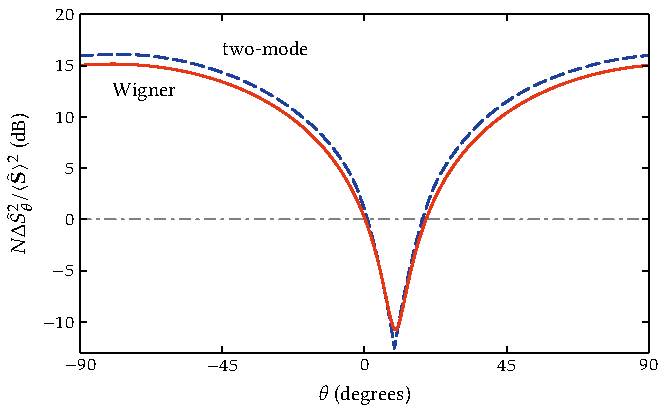
\includegraphics{figures_generated/bec_squeezing/riedel_rotation.pdf}}

    \caption{
    The dependence of the normalized variance on the rotation angle $\theta$ for the Wigner method (red solid line) and the two-mode variational method (dashed blue line, data taken from~\cite{Riedel2010}).
    }
    \label{fig:bec-squeezing:separation:tomography}
\end{figure}

The truncated Wigner approach is applied straightforwardly to this system and allows us to measure the degree of squeezing $xi^2$ according to the formula~\eqnref{bec-squeezing:theory:xi2}, calculating the required spin correlations using the expressions derived in \secref{bec-squeezing:theory}.
Furthermore, we can simulate the observations closer to those used in the experiment, and collect the spin tomography results, as shown in~\figref{bec-squeezing:separation:tomography}.
The maximum degree of squeezing and the corresponding rotation angle corresponds to the minimum of the graph.

The Wigner method shows good agreement with the two-mode variational method~\cite{Li2009}, which was used by the experimental team, and also includes the effect of particle losses.
The two-mode method predictions were taken from~\cite{Riedel2010} and plotted in~\figref{bec-squeezing:separation:tomography} for the sake of comparison \todo{can we do that?}.
The figure demonstrates that the predictions of the two methods for the maximum squeezing angle are nearly identical, and the predictions of the degree of squeezing are close, yet noticeable different ($-10.73\pm0.05\un{dB}$ from the Wigner method as compared with $-12.8\un{dB}$ from the two-mode method).
We believe this is caused by the Wigner method being a more systematic type of approximation with a small parameter, and consequently, more suitable for such complex calculations.

This prediction is hard to verify experimentally, as the technical noise greatly reduces the degree of squeezing (down to $-3.7\un{dB}$), moving it far from the theoretical limit.
The technical noise was not included in the simulations in this thesis, although it can be done similarly to \charef{bec-noise} (since the techincal noise in this experiment has the same nature).
On the other hand, the maximum ``unsqueezing'' (the maximums of the plot in~\figref{bec-squeezing:separation:tomography}), while being irrelevant for practical purposes, can serve as a good experimental check for the two-mode and Wigner methods, as it is much less affected by the technical noise.
The difference of $1\un{dB}$ in the maximum unsqueezing between the two methods should be possible to distinguish.

\begin{figure}
    \centerline{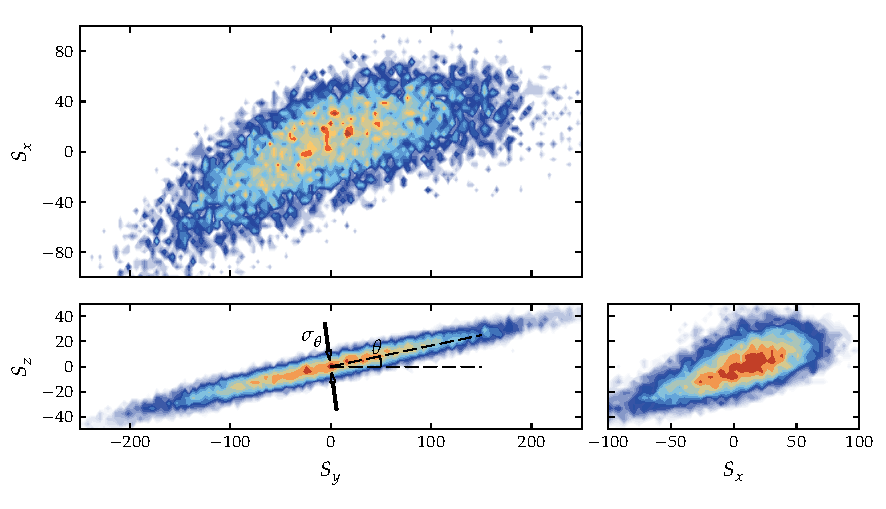
\includegraphics{figures_generated/bec_squeezing/riedel_cloud.pdf}}

    \caption{
    Reconstructed probability distribution for the value of the spin vector projected on $y,z$ plane (a) and spin noise tomography (b).
    The variance $\Delta^2 \hat{S}_\theta$ is connected to the width of the distribution $d_\theta$ in direction $\theta$ (blue line between two arrows in panel (a)) as $2 \sqrt{\Delta^2 \hat{S}_\theta} = d_\theta$.}
    \label{fig:bec-squeezing:separation:cloud-yz}
\end{figure}

We can go further and reconstruct the spin noise distribution using the per-path values of the total spin components, as explained in the end of \secref{bec-squeezing:theory}.
The uncertainty of the total spin in the orthogonal plane is shown in~\figref{bec-squeezing:separation:cloud-yz}.
The shape of the cloud is similar to the one obtained experimentally~\cite{Riedel2010}, and it also serves as a good illustration of the physical meaning of the maximum degree of squeezing and the corresponding rotation angle.

It is interesting to look at all three projections of the cloud, shown in~\figref{bec-squeezing:separation:cloud-yz}.
It is clearly seen that indeed the direction used to measure the squeezing in the experiment is indeed the best one, and the cloud is much wider in other directions.

% =============================================================================
\section{Squeezing near a Feshbach resonance}
% =============================================================================

In the previous section we have discussed an experiment where squeezing was achieved with component-dependent potentials, which helped to reduce the inter-component interaction.
The same effect can be achieved differently~--- by manipulating the external magnetic field near a Feshbach resonance for a chosen pair of hyperfine states.
This allows one to vary the interaction in a wide range with relative ease.
The downside of this approach is a significant increase of the inter-component nonlinear loss rate accompanying the change in the interaction strength.
This results in the destruction of the squeezing as the two components interfere with each other and lose coherence.

The truncated Wigner approach allows us to investigate the combined effect of a reduced interaction strength and increased losses.
In this section we will consider a hypothetical interferometry experiment with two hyperfine states of \Rb{} and demonstrate how with the help of the Wigner method we can pick the optimal value of the magnetic field that leads to the maximum squeezing.

The experiment follows the general scheme used in this and the previous chapters.
We start from a \abbrev{bec} of $N = 55000$ \Rb{} atoms in the hyperfine state ${\ket{F=1,\, m_F=+1}}$ in a cigar-shaped trap with the frequencies $f_x = f_y = 97.0\un{Hz}$ and $f_z = 11.69\un{Hz}$.
The first $\pi/2$-pulse creates an equal superposition of two states, ${\ket{F=1,\, m_F=+1}}$ and ${\ket{F=2,\, m_F=-1}}$.
The external magnetic field of strength $B \approx B_0$ is applied, where $B_0 = 9.1047\un{G}$ corresponds to the Feshbach resonance for the two hyperfine states used~\cite{Kaufman2009}.
We then investigate the time dependence of the maximum degree of spin squeezing.
Intra-component interaction strengths do not depend on the external magnetic field, and are taken to be $a_{11} = 100.4\,r_B$ and $a_{22} = 95.44\,r_B$.

The dependence of the inter-component interaction and loss rate can be described with a single equation for the complex scattering length~\cite{Kaufman2009}
\begin{eqn}
    a(B)
    = a_{\mathrm{bg}} \left(
        1 - \frac{\Delta B}{(B - B_0) - i \gamma_B / 2}
        \right),
\end{eqn}
where $a_{\mathrm{bg}}$ is the background scattering length, $\Delta B$ is the resonance width, and $\gamma_B$ is the decay width.
For a given $B$, the real part of this value acts as the $s$-wave scattering length $a_{12}$ in~\eqnref{bec-noise:system:g}:
\begin{eqn}
\label{eqn:bec-squeezing:feshbach:g}
    g_{12}(B)
    = \frac{4 \pi \hbar^2 \Real a(B)}{m}
    = \frac{4 \pi \hbar^2 a_{\mathrm{bg}}}{m} \left(
        1 - \frac{\Delta B (B - B_0)}{(B - B_0)^2 + \gamma_B^2 / 4}
    \right),
\end{eqn}
and the imaginary part can be connected to the loss rate by substituting it into~\eqnref{bec-noise:system:g} as well and comparing the resulting expression with the corresponding loss term in~\eqnref{bec-noise:mean-field:cgpes-simplified}:
\begin{eqn}
\label{eqn:bec-squeezing:feshbach:gamma}
    \gamma_{12}(B)
    = -\frac{8 \pi \hbar \Imag a(B)}{m}
    = \frac{4 \pi \hbar a_{\mathrm{bg}} \Delta B \gamma_B}{(B - B_0)^2 + \gamma_B^2 / 4}.
\end{eqn}

\begin{figure}
    \centerline{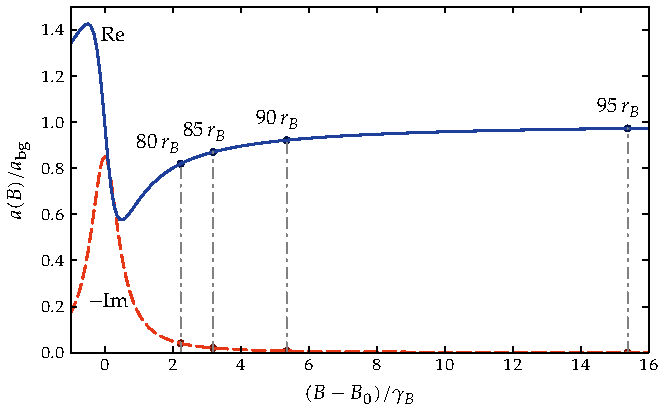
\includegraphics{figures_generated/bec_squeezing/feshbach_scattering.pdf}}

    \caption[Inter-component scattering lenth and loss rate near a Feshbach resonance]{
    Real (blue solid line) and imaginary (red dashed line, negated value is plotted for compactness) parts of the complex scattering length near the Feshbach resonance at $B_0 = 9.1047\un{G}$.
    Four pairs of points show the distances from the resonance chosen for the simulation.
    }%endcaption

    \label{fig:bec-squeezing:feshbach:scattering}
\end{figure}

For the Feshbach resonance we use the reported parameters are $\Delta B = 2\times10^{-3}\un{G}$, $\gamma_B = 4.7\times10^{-3}\un{G}$, and $a_{\mathrm{bg}} = 97.7\,r_B$~\cite{Kaufman2009}.
The behavior of the real and imaginary parts of $a(B)$ near the resonance is shown in~\figref{bec-squeezing:feshbach:scattering}.
From the equations above, as well as from the figure, it is obvious that the minimum inter-species scattering length is achieved when $B - B_0 = 0.5 \gamma_B$.
Unfortunately, this value also corresponds to a relatively large value of the imaginary part, and, correspondingly, the loss rate.
Therefore, we pick the values of $B$ further from the resonance, as displayed in the figure, where the interaction is somewhat stronger, but the loss rate is much lower.
The equations~\eqnref{bec-squeezing:feshbach:g} and~\eqnref{bec-squeezing:feshbach:gamma} give us the following values for the simulation:
\begin{eqn}
    B - B_0 & = 2.24 \gamma_B, \quad
        a_{12} = 80.0\,r_B, \quad \gamma_{12} = 3.85\times10^{-12}\un{cm^3/s},\\
    B - B_0 & = 3.20 \gamma_B, \quad
        a_{12} = 85.0\,r_B, \quad \gamma_{12} = 1.93\times10^{-12}\un{cm^3/s},\\
    B - B_0 & = 5.35 \gamma_B, \quad
        a_{12} = 90.0\,r_B, \quad \gamma_{12} = 7.00\times10^{-13}\un{cm^3/s},\\
    B - B_0 & = 15.4 \gamma_B, \quad
        a_{12} = 95.0\,r_B, \quad \gamma_{12} = 8.53\times10^{-14}\un{cm^3/s}.
\end{eqn}

\begin{figure}
    \centerline{%
    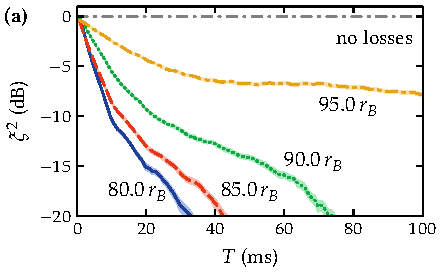
\includegraphics{figures_generated/bec_squeezing/feshbach_squeezing_no_losses.pdf}%
    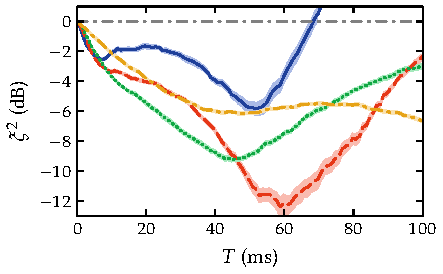
\includegraphics{figures_generated/bec_squeezing/feshbach_squeezing.pdf}}

    \caption[Spin squeezing near a Feshbach resonance]{
    Truncated Wigner simulations of the squeezing in the vicinity of the $B_0 = 9.1047\un{G}$ Feshbach resonance in \Rb{} with different values of the external magnetic field, with \textbf{(a)}~losses turned off, and \textbf{(b)}~inter-component $1,2$-losses turned on.
    Results corresponding to the scattering lengths $a_{12}=80.0\,r_B$ (blue solid line), $a_{12}=85.0\,r_B$ (red dashed line), $a_{12}=90.0\,r_B$ (green dotted line), and $a_{12}=95.0\,r_B$ (yellow dash-dotted line) are plotted.
    The same-colored bands show the estimated sampling error.}%endcaption

    \label{fig:bec-squeezing:feshbach:squeezing}
\end{figure}

First, we perform the simulations with $\gamma_{12}$ set to zero in order to test the squeezing in ideal conditions.
As expected, the lower $a_{12}$ is, the stronger squeezing is reachable, as shown in~\figref{bec-squeezing:feshbach:squeezing},~(a).

With the inclusion of the inter-component losses, the picture is different.
Feshbach tuning to $a_{12} = 85.0\,r_B$ ensures the best squeezing of the four variants ($-12\un{dB}$ at $60\un{ms}$), whereas long lasting squeezing is predicted for the variant with $a_{12} = 95.0\,r_B$ (\figref{bec-squeezing:feshbach:squeezing},~(b)).
In practice, it is possible to run the simulation for other values of $B$, thus finding the ideal balance between the interaction strength and the loss rate which produces the maximum squeezing.

